\documentclass[english,DIV=13]{scrartcl}

\usepackage[utf8x]{inputenc}
\usepackage[T1]{fontenc}
\usepackage{lmodern}
\usepackage[binary-units=true]{siunitx}
% Color
% cfr http://en.wikibooks.org/wiki/LaTeX/Colors
\usepackage{color}
\usepackage[usenames,dvipsnames,svgnames,table]{xcolor}
\definecolor{dkgreen}{rgb}{0.25,0.7,0.35}
\definecolor{dkred}{rgb}{0.7,0,0}
\usepackage{graphicx}
\usepackage{url}
\usepackage{tikz}
\usepackage{pgfplots}
\usepackage{microtype}
\usepackage{xspace}

\usepackage{hyperref}
\usepackage{todonotes}
\usepackage{epstopdf}

\usepackage{multirow}
\usepackage{tabularx} % tabular with automatic line-break
\newcolumntype{Y}{>{\centering\arraybackslash}X} % centered column

\newcommand{\matlab}{\textsc{Matlab}}

% Math symbols
\usepackage{amsmath}
\usepackage{amssymb}
\usepackage{amsthm}
\DeclareMathOperator*{\argmin}{arg\,min}
\DeclareMathOperator*{\argmax}{arg\,max}

% Unit vectors
\usepackage{esint}
\usepackage{esvect}
\newcommand{\kmath}{k}
\newcommand{\xunit}{\hat{\imath}}
\newcommand{\yunit}{\hat{\jmath}}
\newcommand{\zunit}{\hat{\kmath}}
\newcommand{\uunit}{\hat{\umath}}

% Elec
\newcommand{\B}{\vec B}
\newcommand{\E}{\vec E}
\newcommand{\EMF}{\mathcal{E}}
\newcommand{\perm}{\varepsilon} % permittivity

\newcommand{\bigoh}{\mathcal{O}}
\newcommand\eqdef{\triangleq}

\DeclareMathOperator{\newdiff}{d} % use \dif instead
\newcommand{\dif}{\newdiff\!}
\newcommand{\fpart}[2]{\frac{\partial #1}{\partial #2}}
\newcommand{\ffpart}[2]{\frac{\partial^2 #1}{\partial #2^2}}
\newcommand{\fdpart}[3]{\frac{\partial^2 #1}{\partial #2\partial #3}}
\newcommand{\fdif}[2]{\frac{\dif #1}{\dif #2}}
\newcommand{\ffdif}[2]{\frac{\dif^2 #1}{\dif #2^2}}
\newcommand{\constant}{\ensuremath{\mathrm{cst}}}
\newcommand{\norm}[1]{\left\lVert#1\right\rVert}

\usepackage{babel}
% Listing
% always put it after babel
% http://tex.stackexchange.com/questions/100717/code-in-lstlisting-breaks-document-compile-error
\usepackage{listings}

% Put caption after babel
\usepackage{caption}
\usepackage{subcaption}

\definecolor{mygreen}{rgb}{0,0.6,0}
\definecolor{mygray}{rgb}{0.5,0.5,0.5}
\definecolor{mymauve}{rgb}{0.58,0,0.82}
\lstset{ %
  language=Matlab,
  backgroundcolor=\color{white},   % choose the background color; you must add \usepackage{color} or \usepackage{xcolor}
  basicstyle=\footnotesize,        % the size of the fonts that are used for the code
  breakatwhitespace=false,         % sets if automatic breaks should only happen at whitespace
  breaklines=true,                 % sets automatic line breaking
  captionpos=b,                    % sets the caption-position to bottom
  commentstyle=\color{mygreen},    % comment style
  deletekeywords={...},            % if you want to delete keywords from the given language
  escapeinside={\%*}{*)},          % if you want to add LaTeX within your code
  extendedchars=true,              % lets you use non-ASCII characters; for 8-bits encodings only, does not work with UTF-8
  frame=single,	                   % adds a frame around the code
  keepspaces=true,                 % keeps spaces in text, useful for keeping indentation of code (possibly needs columns=flexible)
  keywordstyle=\color{blue},       % keyword style
  otherkeywords={*,...},           % if you want to add more keywords to the set
  numbers=none,                    % where to put the line-numbers; possible values are (none, left, right)
  numbersep=5pt,                   % how far the line-numbers are from the code
  numberstyle=\tiny\color{mygray}, % the style that is used for the line-numbers
  rulecolor=\color{black},         % if not set, the frame-color may be changed on line-breaks within not-black text (e.g. comments (green here))
  showspaces=false,                % show spaces everywhere adding particular underscores; it overrides 'showstringspaces'
  showstringspaces=false,          % underline spaces within strings only
  showtabs=false,                  % show tabs within strings adding particular underscores
  stepnumber=2,                    % the step between two line-numbers. If it's 1, each line will be numbered
  stringstyle=\color{mymauve},     % string literal style
  tabsize=2,	                   % sets default tabsize to 2 spaces
  title=\lstname                   % show the filename of files included with \lstinputlisting; also try caption instead of title
}

\KOMAoptions{DIV=last}




% Definition to put a bar under a letter/word (to use with matrix)
\usepackage{accents}
\newcommand{\ubar}[1]{\underaccent{\bar}{#1}}
\newcommand{\uvec}[1]{\ubar{#1}}
\newcommand{\umatrix}[1]{\ubar{\ubar{#1}}}

\titlehead{}
\subject{LINMA 1731 --- Stochastic processes}
\title{Bearings-only tracking problem}
\subtitle{}
\author{\textsc{Cassiers} Gaëtan \and \textsc{Losseau} Bruno}
\date{\today}

\begin{document}
\maketitle


\section*{Question 1}
\subsection*{Deriving $\umatrix{F}$ and $\uvec{U}$}

We start by studying the making a discretization of a movemement process in 1D, with the
variable $x(t)$. If we denode $x_k = x(Tk)$ (with $T$ a given discretization step), we
get
\begin{align*}
    x_{k+1} &= x_k + T\dot{x}_k + \int_{Tk}^{T(k+1)}\int_{Tk}^{t}\ddot{x}(t)\dif t\dif t' \\
    \dot{x}_{k+1} &=  \dot{x}_k + \int_{Tk}^{T(k+1)}\dot{x}(t)\dif t.
\end{align*}
This is a simple discrete-time state model, if we consider that the terms which depends of $\ddot{x}$
are an input signal.
We can generalize this equation to the relative state vector $\uvec{x} = \uvec{x}^t - \uvec{x}^o$:
\[\uvec{x}_{k+1} = \umatrix{F}\uvec{x}_k - \uvec{U}_{k,k+1} + \uvec{\epsilon}_k\]
with
\begin{itemize}
    \item The matrix
        \[\umatrix{F} =
        \begin{pmatrix}
            1 & 0 & T & 0 \\
            0 & 1 & 0 & T \\   
            0 & 0 & 1 & 0 \\
            0 & 0 & 0 & 1   
        \end{pmatrix}
        \]
    \item $\uvec{\epsilon}_k$ the variation of position and of velocity of the target caused by the
acceleration of the target,
    \item $\uvec{U}_{k,k+1}$ the variation of position and velocity of
the observer caused by the acceleration of the observer.
\end{itemize}

\subsection*{Deriving $h(\ubar{x})$}
Following its definition given in the statement and unsing the notation $\uvec{x}(i)$
for the $i$-th element of the vector $\uvec{x}$:
\begin{align*}
    h(\uvec{x}_k) &= \text{atan2}(\uvec{x}_k(1), \uvec{x}_k(2)) \\
    &= \begin{cases}
        \arctan\frac{\uvec{x}_k(1)}{\uvec{x}_k(2)} & \text{if $\uvec{x}_k(2) > 0$} \\
        \arctan\frac{\uvec{x}_k(1)}{\uvec{x}_k(2)}+\pi & \text{if $\uvec{x}_k(2) < 0$ and $\uvec{x}_k(1) \geq 0$} \\
        \arctan\frac{\uvec{x}_k(1)}{\uvec{x}_k(2)}-\pi & \text{if $\uvec{x}_k(2) < 0$ and $\uvec{x}_k(1) < 0$} \\
        0 & \text{if $\uvec{x}_k(2) \geq 0$ and $\uvec{x}_k(1) = 0$} \\
        \pi & \text{if $\uvec{x}_k(2) < 0$ and $\uvec{x}_k(1) = 0$}
    \end{cases}
\end{align*}


\section*{Question 2}

Results for question 2:
\begin{center}
   \includegraphics[width=0.49\textwidth]{img/q2_1.eps}
   \includegraphics[width=0.49\textwidth]{img/q2_2.eps}
   \includegraphics[width=0.49\textwidth]{img/q2_3.eps}
   \includegraphics[width=0.49\textwidth]{img/q2_4.eps}
\end{center}


\section*{Question 3}
\begin{figure}
   \caption{\label{q3a} }
   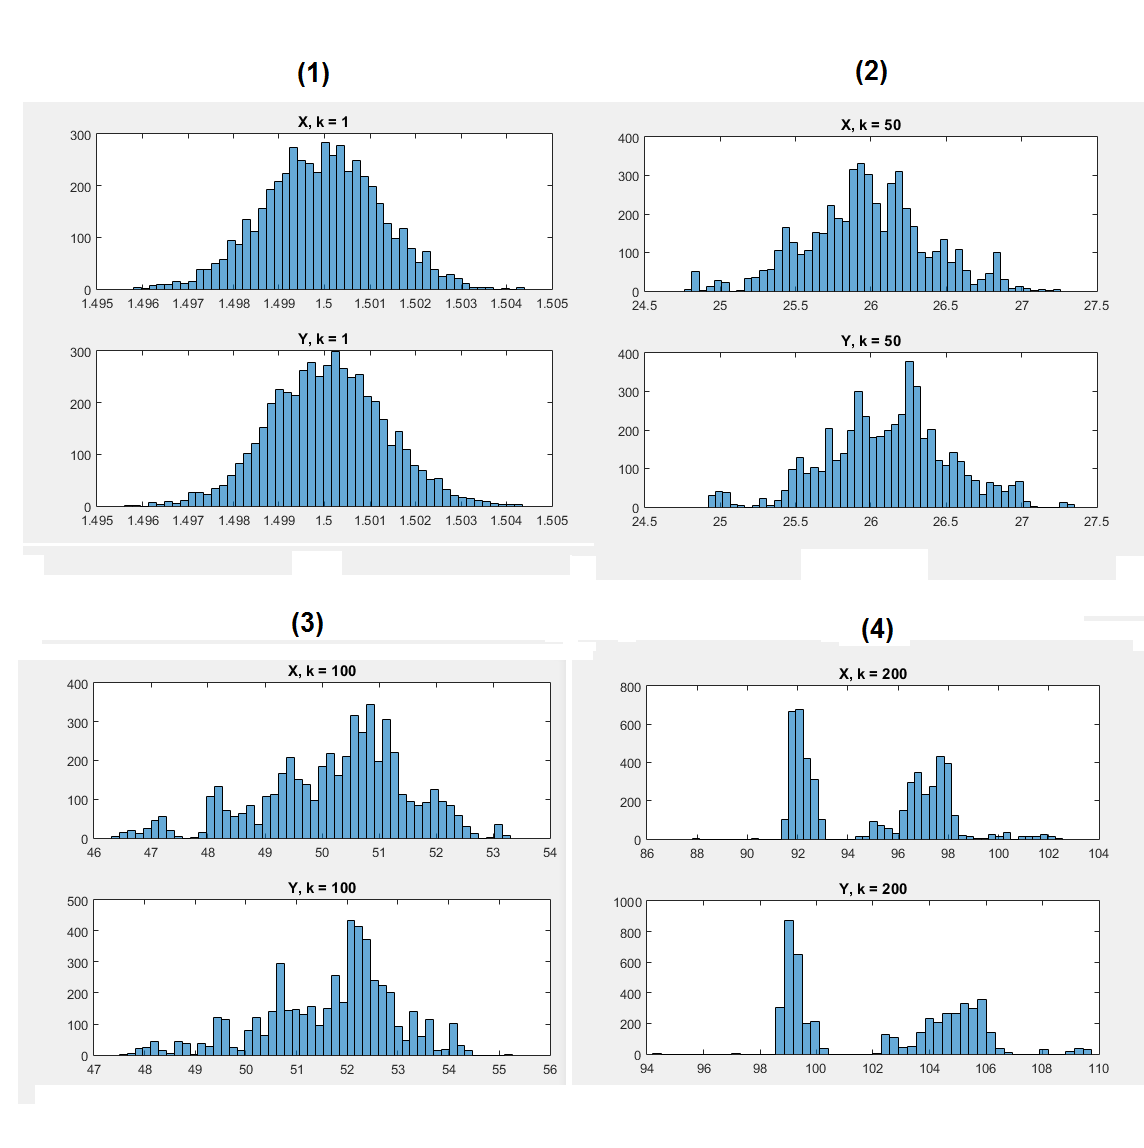
\includegraphics[width=\textwidth,height=\textheight,keepaspectratio]{q3a.png}
\end{figure}
\begin{figure}
\begin{center}
   \caption{\label{q3b} }
   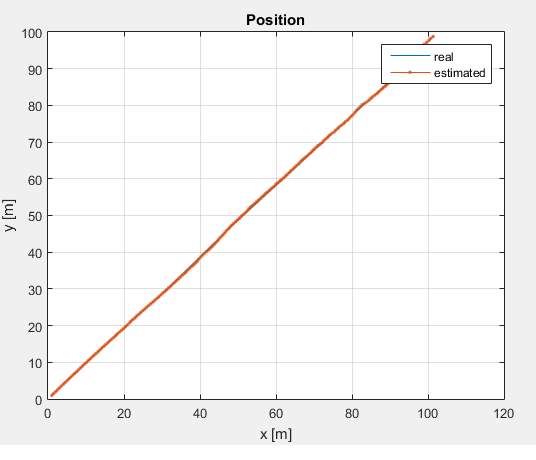
\includegraphics[width=10cm,height=\textheight,keepaspectratio]{q3b.png}
\end{center}
\end{figure}


\section*{Question 4}
\begin{figure}
   \caption{\label{q4} }
   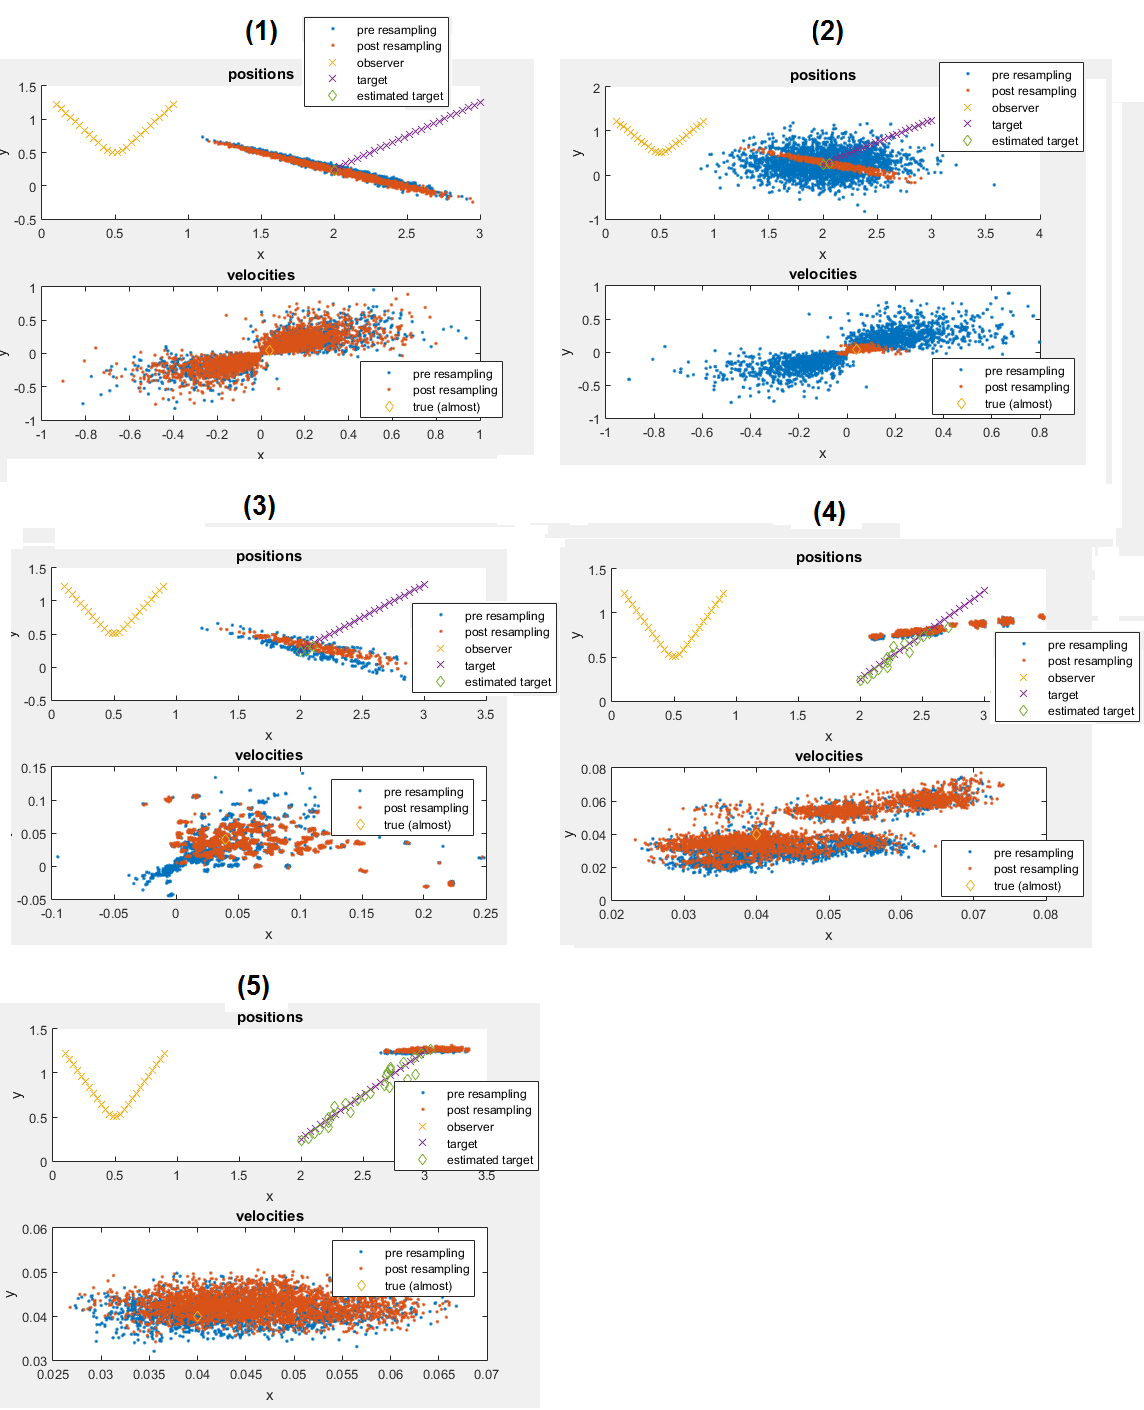
\includegraphics[width=\textwidth,height=\textheight,keepaspectratio]{q4.png}
\end{figure}

\section*{Question 5}


\section*{Question 6}


\section*{Codes matlab}
\lstinputlisting{../matlab/q2.m}


\end{document}
